% Drop-in experiment section for the MotionScorer / nuGuidance paper.
% Required in the parent project: graphicx, booktabs, amsmath, xcolor.
% The parent project must define \methodname{} and the cited bibliography keys.

\providecommand{\est}[1]{\textcolor{black}{#1}}
\providecommand{\blankresult}{\phantom{00.000}}

\subsection{Setup}
\label{sec:setup}

\paragraph{Backbone and supervision.}
All VLM-based methods start from the same Qwen2.5-VL-7B checkpoint used as the
base model of DriveCritic, before its task-specific trajectory-evaluation
adaptation \citep{song2025drivecritic}. Direct prompting, fixed-query readout,
plain query readout, and \methodname{} keep every backbone parameter frozen.
The LoRA and full-backbone SFT baselines start from the identical checkpoint
but update low-rank adapters or all backbone parameters, respectively.
Full teacher and implementation details appear in
App.~\ref{app:experiment_settings}.

\paragraph{Benchmarks.}
Pseudo-score training and validation use public NAVSIM and Pseudo-Simulation
scene--trajectory pools \citep{dauner2024navsim,cao2025pseudosim}. External
human-alignment evaluation uses the public WOD-E2E validation set
\citep{xu2025wode2e}, which provides three candidate trajectories per
long-tail driving segment together with existing expert ratings on a
$0$--$10$ scale. These ratings form a locked external test and are never used
for training, prompt selection, hyperparameter tuning, checkpoint selection,
seed selection, or output calibration.

The semantic-regime analysis uses pre-registered subsets defined
automatically from the fixed teacher score, available rule outputs, and
existing human ratings; no item is manually selected according to model
performance. No new human annotation is collected for any experiment.

\paragraph{Metrics and protocol.}
On WOD-E2E, we report pairwise accuracy, Kendall's $\tau_b$, NDCG@3, and
fixed-scale MAE. Native-channel analysis additionally reports the effective
number of score levels, prompt sensitivity, and valid-output rate.
Semantic-regime analysis reports subgroup MAE, TranscendRate, and worst-group
MAE. Causal interventions report paired performance changes and held-out
$\rho_{\mathrm{TCD}}$. On held-out pseudo-labelled data, we report RMSE and
Spearman rank correlation coefficient (SRCC) against the automatic teacher.
Adaptation cost, memory, latency, and preservation of the backbone's original
abilities are reported separately in the appendix.


\subsection{Main Result: Public Human-Aligned Trajectory Scoring}
\label{sec:wod_human_alignment}

Table~\ref{tab:wod_human_alignment} evaluates whether scores learned only from
automatic supervision agree with the existing WOD-E2E human ratings. The
plain-readout versus direct-prompting comparison tests whether the frozen
attention interface is a better scoring channel, while the LoRA comparison
measures the remaining gap to weight modification.

\begin{table*}[t]
    \centering
    \small
    \setlength{\tabcolsep}{4.2pt}
    \renewcommand{\arraystretch}{1.10}
    \caption{
        Public human-aligned trajectory scoring on WOD-E2E.
        All learned methods use zero task-specific human labels during training
        and model selection.
    }
    \label{tab:wod_human_alignment}
    \resizebox{\textwidth}{!}{
    \begin{tabular}{lccccccc}
        \toprule
        Method
        & \shortstack{Backbone\\updated}
        & Training supervision
        & \shortstack{Human labels\\for training}
        & \shortstack{Pairwise\\Acc. (\%) $\uparrow$}
        & Kendall $\tau_b$ $\uparrow$
        & NDCG@3 $\uparrow$
        & \shortstack{Fixed-scale\\MAE $\downarrow$}
        \\
        \midrule

        Imitation score (negative ADE/FDE)
        & --
        & Logged-trajectory geometry
        & 0
        & \est{64.5}
        & \est{0.28}
        & \est{0.87}
        & --
        \\

        Trajectory-only MLP scorer
        & --
        & Automatic pseudo scores
        & 0
        & \est{61.0}
        & \est{0.21}
        & \est{0.85}
        & \est{2.64}
        \\

        Same-backbone direct prompting
        & No
        & None
        & 0
        & \est{54.2}
        & \est{0.07}
        & \est{0.81}
        & \est{2.92}
        \\

        Plain query readout
        & No
        & Automatic pseudo scores
        & 0
        & \est{66.8}
        & \est{0.33}
        & \est{0.89}
        & \est{2.31}
        \\

        Same-backbone LoRA scorer
        & Yes
        & Automatic pseudo scores
        & 0
        & \est{71.5}
        & \est{0.42}
        & \est{0.92}
        & \est{2.02}
        \\

        \midrule
        \textbf{\methodname{} (Ours)}
        & \textbf{No}
        & \textbf{Automatic pseudo scores}
        & \textbf{0}
        & \est{70.3}
        & \est{0.40}
        & \est{0.91}
        & \est{2.10}
        \\
        \bottomrule
    \end{tabular}
    }
\end{table*}

As shown in Table~\ref{tab:wod_human_alignment}, \methodname{} raises pairwise
accuracy from 54.2\% with direct prompting to 70.3\% and NDCG@3 from 0.81 to
0.91; it also improves over the plain query readout by 3.5 percentage points
and reduces MAE from 2.31 to 2.10. Its pairwise accuracy is only 1.2 points
below the same-backbone LoRA scorer (70.3\% vs.\ 71.5\%) without updating the
backbone, showing that most of the human-aligned scoring ability can be
recovered through the frozen query interface.


\subsection{Main Result: Matched-Fit Readout Comparison}
\label{sec:matched_fit}

Table~\ref{tab:matched_fit} isolates the contribution of
teacher-conditioned deflection. Every trainable row uses the same correct
pseudo scores in its endpoint scoring loss. In the permutation control, only
the targets used to construct the deflection criterion are permuted.

\begin{table*}[t]
    \centering
    \small
    \setlength{\tabcolsep}{3.4pt}
    \renewcommand{\arraystretch}{1.10}
    \caption{
        Matched pseudo-score fit and public cross-domain human generalization.
        Plain query readout and \methodname{} share the same frozen checkpoint,
        supervision, capacity, optimization, and training budget.
    }
    \label{tab:matched_fit}
    \resizebox{\textwidth}{!}{
    \begin{tabular}{lcccccccc}
        \toprule
        Variant
        & \shortstack{Learn\\queries $E$}
        & \shortstack{TCD\\target}
        & \shortstack{Criterion\\location}
        & \shortstack{Pseudo-val.\\RMSE $\downarrow$}
        & \shortstack{Pseudo-val.\\SRCC $\uparrow$}
        & \shortstack{WOD pairwise\\Acc. (\%) $\uparrow$}
        & \shortstack{WOD\\NDCG@3 $\uparrow$}
        & \shortstack{Held-out\\$\rho_{\mathrm{TCD}}\uparrow$}
        \\
        \midrule

        Fixed/random queries, scalar head only
        & No
        & --
        & --
        & \est{0.142}
        & \est{0.712}
        & \est{61.5}
        & \est{0.86}
        & \est{3.1}
        \\

        Plain query readout $(\lambda=0)$
        & Yes
        & --
        & --
        & \est{0.096}
        & \est{0.888}
        & \est{66.8}
        & \est{0.89}
        & \est{6.4}
        \\

        TCD with permuted pseudo scores
        & Yes
        & Permuted
        & Attention branch
        & \est{0.097}
        & \est{0.885}
        & \est{66.3}
        & \est{0.89}
        & \est{6.1}
        \\

        TCD on full score-query state
        & Yes
        & Correct
        & Full state
        & \est{0.095}
        & \est{0.889}
        & \est{67.9}
        & \est{0.90}
        & \est{6.9}
        \\

        Same-backbone LoRA scorer
        & --
        & --
        & --
        & \est{0.089}
        & \est{0.901}
        & \est{71.5}
        & \est{0.92}
        & --
        \\

        \midrule
        \textbf{\methodname{} (Ours)}
        & \textbf{Yes}
        & \textbf{Correct}
        & \textbf{Attention branch}
        & \est{0.095}
        & \est{0.891}
        & \est{70.3}
        & \est{0.91}
        & \est{8.7}
        \\
        \bottomrule
    \end{tabular}
    }
\end{table*}

Table~\ref{tab:matched_fit} shows nearly matched pseudo-score fit between
\methodname{} and the plain readout (0.095 vs.\ 0.096 RMSE and 0.891 vs.\ 0.888
SRCC), while \methodname{} improves WOD pairwise accuracy from 66.8\% to
70.3\% and increases held-out $\rho_{\mathrm{TCD}}$ from 6.4 to 8.7. The
permuted-target and full-state controls reach only 66.3\% and 67.9\%
pairwise accuracy, respectively, indicating that the gain depends on the
correctly conditioned criterion acting on the exact attention branch rather
than on generic latent regularization.


\subsection{Inner Comparison}
\label{sec:inner_comparison}

The cross-method results establish whether \methodname{} is externally
competitive. We next hold the backbone, rendered inputs, pseudo labels, and
evaluation protocol fixed, and test three narrower claims: whether the native
numeric channel remains limiting under stronger prompting controls; whether
the gain concentrates in semantically difficult teacher--human disagreement
regimes; and whether the learned context-attention pattern causally contributes
to the score. Exact values behind all three visualizations are retained in
App.~\ref{app:numeric_visualizations}, and full constructions appear in
App.~\ref{app:inner_comparison}.


\subsubsection{Native Scoring Channel}
\label{sec:native_channel}

All prompting controls use the same frozen backbone, multimodal input, and
evaluation rubric; they differ only in how the native language channel is
elicited.

\begin{figure*}[t]
    \centering
    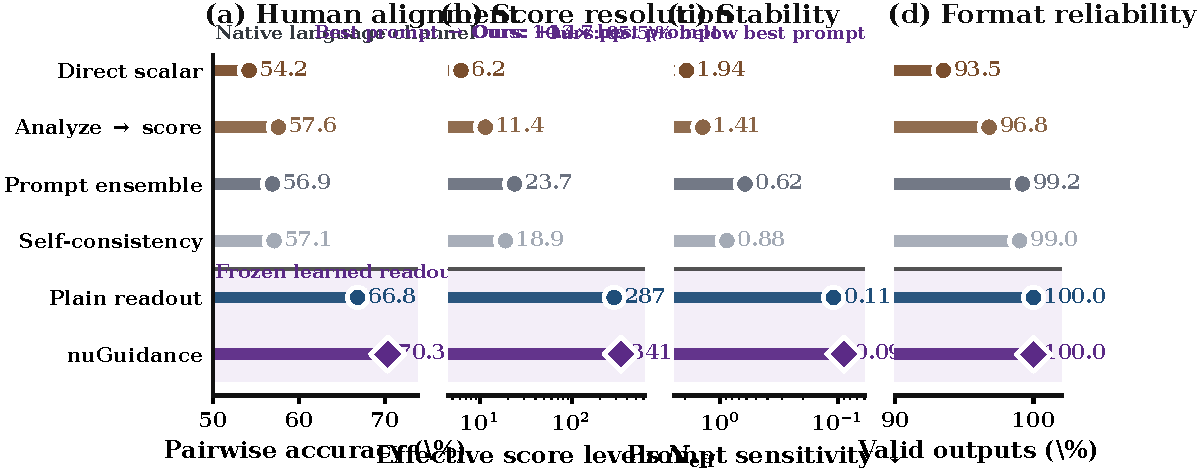
\includegraphics[width=0.99\textwidth]{figures/fig_native_scoring_channel.pdf}
    \caption{\textbf{Stronger prompting does not repair the native scoring channel.}
    The same methods are aligned across four small multiples: human-aligned
    pairwise accuracy, effective score resolution, prompt sensitivity, and
    valid-output rate. Prompting controls remain low-resolution and
    prompt-sensitive even when ensembling or repeated sampling improves format
    validity. The frozen learned readouts move to a distinct operating regime,
    with \methodname{} attaining 70.3\% pairwise accuracy, 341 effective score
    levels, 0.09 sensitivity, and 100\% valid outputs. Exact NDCG@3 values are
    reported in App.~\ref{tab:native_channel_numeric}.}
    \label{fig:native_scoring_channel}
\end{figure*}

Figure~\ref{fig:native_scoring_channel} rules out an under-optimized direct
prompt as the main explanation for the readout gain. Analyze-then-score is the
strongest prompting baseline at 57.6\% pairwise accuracy, whereas
\methodname{} reaches 70.3\%, a 12.7-point gain. More importantly, the best
prompt ensemble exposes only 23.7 effective score levels and remains at 0.62
prompt sensitivity; \methodname{} exposes 341 levels---14.4$\times$ more---and
reduces sensitivity to 0.09. The plain readout already produces the same
qualitative transition, and TCD improves its accuracy by a further 3.5 points.
Thus, ensembling and repeated decoding improve formatting, but do not close the
gap created by the textual numeric channel.


\subsubsection{Semantic Disagreement Regimes}
\label{sec:disagreement_regimes}

Overall performance can conceal whether an evaluator succeeds on the cases
that motivate semantic scoring. We therefore partition WOD-E2E automatically
using the fixed Scheme-B teacher score, public rule outputs, and existing human
ratings. No additional annotation or manual case selection is introduced.

\begin{figure*}[t]
    \centering
    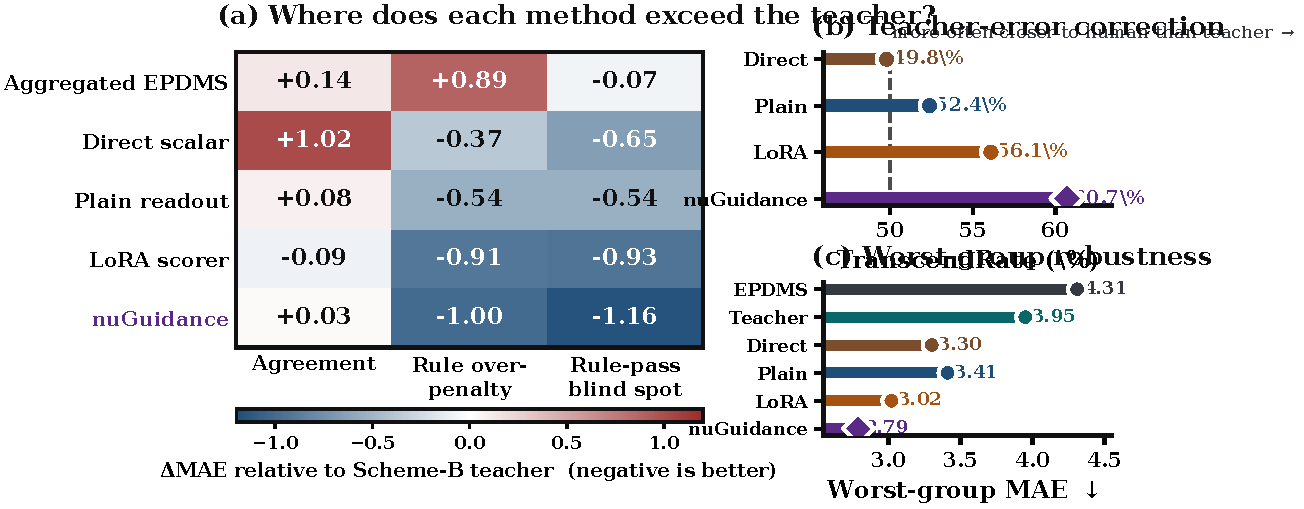
\includegraphics[width=0.99\textwidth]{figures/fig_semantic_disagreement.pdf}
    \caption{\textbf{The gain concentrates where the automatic teacher and humans disagree.}
    Left: MAE change relative to the Scheme-B teacher in three pre-registered
    regimes; negative values mean closer agreement with human ratings. Right:
    TranscendRate and worst-group MAE summarize teacher-error correction and
    robustness. \methodname{} achieves the largest teacher-relative gains on
    rule over-penalty ($-1.00$ MAE) and rule-pass blind spots ($-1.16$), the
    highest TranscendRate (60.7\%), and the lowest worst-group MAE (2.79).}
    \label{fig:semantic_disagreement}
\end{figure*}

Figure~\ref{fig:semantic_disagreement} separates faithful teacher fitting from
semantic correction. Relative to the teacher, \methodname{} is essentially
unchanged on the agreement subset ($+0.03$ MAE), but improves by 1.00 point on
rule over-penalty items and by 1.16 points when all represented rules pass yet
the teacher still overestimates human quality. Its 60.7\% TranscendRate exceeds
the plain readout's 52.4\% and LoRA's 56.1\%, while its 2.79 worst-group MAE is
the best result. The asymmetry is the intended pattern: the method does not
merely smooth the teacher scale, but gains specifically on the regimes in which
the rule bottleneck is informative and structurally limiting.


\subsubsection{Causal Readout Interventions}
\label{sec:causal_interventions}

We intervene on the exact context-attention branch used by the filtering
criterion. A single trained \methodname{} checkpoint and scalar head are held
fixed, and no intervention is followed by retraining.

\begin{figure*}[t]
    \centering
    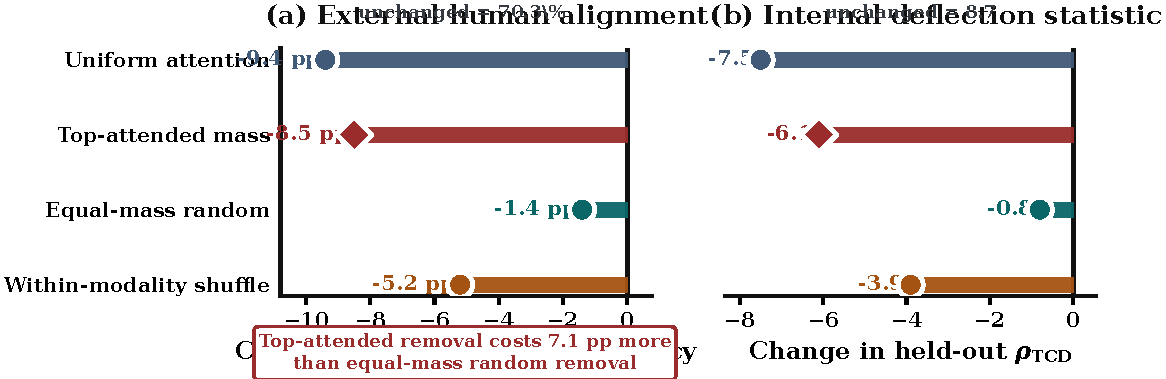
\includegraphics[width=0.98\textwidth]{figures/fig_causal_interventions.pdf}
    \caption{\textbf{The learned attention pattern is functionally responsible for the score.}
    Both panels report changes from the unchanged checkpoint, whose WOD
    pairwise accuracy and held-out deflection are 70.3\% and 8.7. Left:
    intervention-induced accuracy change. Right: change in
    $\rho_{\mathrm{TCD}}$. Removing top-attended evidence costs 8.5 percentage
    points, 7.1 points more than removing equal attention mass at random, and
    the deflection statistic falls in the same ordering. Values are paired
    point estimates; exact absolute RMSE, NDCG@3, accuracy, and deflection are
    reported in App.~\ref{tab:attention_interventions_numeric}.}
    \label{fig:causal_interventions}
\end{figure*}

Figure~\ref{fig:causal_interventions} provides the mechanism test that an
attention visualization alone cannot. Uniform attention reduces pairwise
accuracy by 9.4 points and deflection by 7.5. Suppressing the highest-attended
mass causes an 8.5-point accuracy drop and a 6.1-point deflection drop, whereas
suppressing equal mass at random costs only 1.4 and 0.8, respectively.
Within-modality shuffling gives an intermediate degradation. Because every
intervention reuses the identical checkpoint and scalar head, the 7.1-point
top-versus-random contrast isolates position-specific evidence selected by the
learned readout rather than generic loss of attention mass.
